\section{Kurven und Flächen}%
\label{kuf:sec:kurven_und_flaechen}

\subsection{Bézierkurven}%
\label{kuf:sub:bezierkurven}
\begin{itemize}
	\item Aufgebaut aus Bernsteinpolynomen
	\item $b_i$ heißen Stützpunkte
\end{itemize}
\vspace*{-0.5cm}
$$F(u) = \sum_{i=0}^n B_i^n(u)b_i, \text{mit } b_i \in \realnumbers^d$$ 

\subsubsection{Lemma von Bézier}%
\label{kuf:sub:lemma_von_bezier}

\begin{itemize} 
	\item $F(u)$ liegt in der abgeschlossenen konvexen Hülle des Kontrollpolygons
	\item Endpunktinterpolation $F(0) = b_0$ und $F(1) = b_n$
	\item Tangentenbedigung $F'(0) = n(b_1 - b_0) \land F'(1) = n(b_n - b_{n-1})$
	\item Affine Invarianz: Sei $\varphi(x) = Ax + t$ eine affine Abbildung, dann gilt
  $$F(u) = \sum^n_{i=0} B_i^n(u) \varphi(b_i)$$
	\item Variationsreduzierung: Eine Bézier-Kurve wackelt nicht stärker als Kontrollpolygon
\end{itemize}

\subsection{De-Casteljau-Algorithmus}%
\label{kuf:sub:de_casteljau-algorithmus}

Rekursiver Algorithmus zur effizienten Auswertung von Bezierkurven an einzelnen Punkten:
$$B_i^n(u) = u \cdot B_{i-1}^{n-1} (u) + (1 - u) \cdot B_i^{n-1}(u)$$\vspace*{-0.5cm}
\begin{figure}[h]
	\centering
	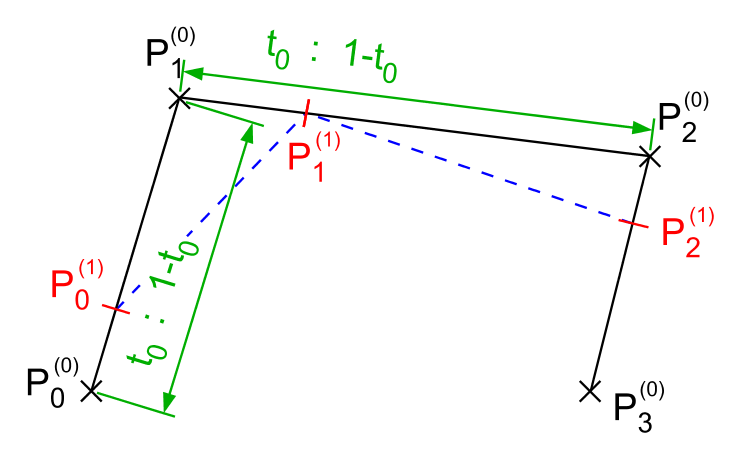
\includegraphics[width=6cm]{images/De_Casteljau_construction_1}
	\caption{https://commons.wikimedia.org/wiki/File:De\_Casteljau\_construction\_1.png}
\end{figure}
\newpage
\subsection{Bézier-Splines}%
\label{kuf:sub:bezier-splines}

\begin{itemize}
	\item Bei hohem Grad beeinflusst jeder Punkt die ganze Kurve $\rightarrow$ schwierig bei Modellierung
	\item Deshalb: Füge mehere Kurven niedrigeren Grades aneinander
\end{itemize}
\textbf{Definition}\\
Stückwise polynomielle Kurve, deren einzelne Abschnitte durch Bézier-Kurven beschrieben sind.\\

\textbf{Stetigkeit}\\
Setze Bézier-Spline $C^2$ stetig fort. Spline $B$ mit $b_i$.
Forsetzung mit Spline $C$ mit $c_i$. Dann gilt
\begin{align*}
  b_n &= c_0\\
  b_n - b_{n-1} &= c_1 - c_0\\
  b_{n-1} + (b_{n-1} -  b_{n-2}) &= c_1 + (c_1 - c_2)
\end{align*}
Damit:
\begin{align*}
	c_0 &= b_n\\
	c_1 &= c_0 + (c_0 - b_{n-1})\\
	c_2 &= c_1 + (c_1 - (b_{n-1} + (b_{n-1} - b_{n-2})))
\end{align*}